\documentclass[border=5pt,tikz]{standalone}
\usepackage{amsmath}
\usetikzlibrary{calc}
\usetikzlibrary{math}
\usetikzlibrary {shapes.geometric} % for star
\usetikzlibrary{bending} % for arrow head angle
\usetikzlibrary{angles,quotes} % for pic (angle labels)
\usetikzlibrary{arrows.meta} % for arrow size
\usetikzlibrary{decorations.pathmorphing,patterns}

\usetikzlibrary {arrows}
\usetikzlibrary{shapes.geometric}
\begin{document}
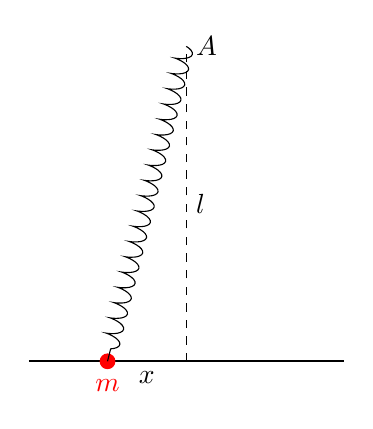
\begin{tikzpicture} %[=>stealth]
    \def\R1{3};
    \def\R2{3};
    \def\theta1{30};
    \def\theta2{40};

    \coordinate (O) at (0, 0);  
    \coordinate (A) at (0, 4);
    \coordinate (M) at (-1, 0);
   
    \draw[dashed] (O) -- node [right] {$l$} (A) node [right] {$A$};
    \draw[thick] (-2, 0) -- (2, 0);    
    \fill[red] (M) circle (0.1cm) node[below, yshift=-0.3em] {$m$};
    \draw[decoration={aspect=0.3, segment length=2mm, amplitude=1mm,coil},decorate] (A) -- (M); 
    \node [below] at (-0.5, 0) {$x$};
\end{tikzpicture}
\end{document}
